\documentclass[12pt]{report}

%%%%%%%%%%%%%%%%%%%%%%%%%%%%%%%%%%%%%%%%%%%%%%%%%%%%%%%%%%%%%%%%%%%%
% package and document formatting stuff
%%%%%%%%%%%%%%%%%%%%%%%%%%%%%%%%%%%%%%%%%%%%%%%%%%%%%%%%%%%%%%%%%%%%

% symbols and math stuff
\usepackage{amsmath,amsthm,amssymb}
\usepackage{tikz}
\usepackage{tkz-graph}
\usetikzlibrary{arrows,%
                petri,%
                topaths}%

\usepackage{tkz-berge}


% math operators
\usepackage{amsopn}

% script and caligraphics
\usepackage{eucal,mathrsfs}

% indexing
\usepackage{makeidx}

\usepackage{enumerate}

% formatting
\usepackage{fullpage}

% links and colors
\usepackage{color}
\usepackage[pdfstartview=FitH,
%             pdfauthor={\myauthor},
%             pdftitle={\mytitle},
            colorlinks,
            linkcolor=reference,
            citecolor=citation,
            urlcolor=e-mail,
            backref]{hyperref}
\usepackage[all]{xy}

\definecolor{todo}{rgb}{.80,.20,.20}
\definecolor{e-mail}{rgb}{0,.40,.80}
\definecolor{reference}{rgb}{.10,.40,.42}
\definecolor{mrnumber}{rgb}{.80,.40,0}
\definecolor{citation}{rgb}{0,.40,.80}

\usepackage{graphicx}

%%%%%%%%%%%%%%%%%%%%%%%%%%%%%%%%%%%%%%%%%%%%%%%%%%%%%%%%%%%%%%%%%%%%
% theorem stuff
%%%%%%%%%%%%%%%%%%%%%%%%%%%%%%%%%%%%%%%%%%%%%%%%%%%%%%%%%%%%%%%%%%%%

\theoremstyle{plain}

\newtheorem{thm}{Theorem}[section]
\newtheorem{defn}[thm]{Definition}
\newtheorem{deflem}[thm]{Definition/Lemma}
\newtheorem{notn}[thm]{Notation}
\newtheorem{convention}[thm]{Convention}
\newtheorem{lem}[thm]{Lemma}
\newtheorem{aside}[thm]{Aside}
\newtheorem{rem}[thm]{Remark}
\newtheorem{ex}[thm]{Example}
\newtheorem{facts}[thm]{Facts}
\newtheorem{cor}[thm]{Corollary}
\newtheorem{conj}[thm]{Conjecture}
\newtheorem{prop}[thm]{Proposition}

\newtheorem{question}[thm]{Question}
\newtheorem{exercise}{Exercise}[section]

%%%%%%%%%%%%%%%%%%%%%%%%%%%%%%%%%%%%%%%%%%%%%%%%%%%%%%%%%%%%%%%%%%%%
% typography stuff
%%%%%%%%%%%%%%%%%%%%%%%%%%%%%%%%%%%%%%%%%%%%%%%%%%%%%%%%%%%%%%%%%%%%

\newcommand{\mb}[1]{\mathbf #1}
\newcommand{\mbb}[1]{\mathbb #1}
\newcommand{\mf}[1]{\mathfrak #1}
\newcommand{\mc}[1]{\mathcal #1}
\newcommand{\ms}[1]{\mathscr #1}
\newcommand{\mcu}[1]{\mathcu #1}
\newcommand{\oper}[1]{\operatorname{#1}}

\newcommand{\da}{\downarrow}
\newcommand{\ra}{\rightarrow}
\newcommand{\hra}{\hookrightarrow}
\newcommand{\dra}{\dashrightarrow}
\newcommand{\la}{\leftarrow}
\newcommand{\lra}{\longrightarrow}

\newcommand{\ov}{\overline}
\newcommand{\til}{\widetilde}
\newcommand{\wh}{\widehat}

\newcommand{\ZZ}{\mathbb{Z}}

\newcommand{\lcm}{\oper{lcm}}

%%%%%%%%%%%%%%%%%%%%%%%%%%%%%%%%%%%%%%%%%%%%%%%%%%%%%%%%%%%%%%%%%%%%
% other stuff
%%%%%%%%%%%%%%%%%%%%%%%%%%%%%%%%%%%%%%%%%%%%%%%%%%%%%%%%%%%%%%%%%%%%

\newcommand{\todo}[1]{\textcolor{todo}{#1}}

%%%%%%%%%%%%%%%%%%%%%%%%%%%%%%%%%%%%%%%%%%%%%%%%%%%%%%%%%%%%%%%%%%%%
% end preamble
%%%%%%%%%%%%%%%%%%%%%%%%%%%%%%%%%%%%%%%%%%%%%%%%%%%%%%%%%%%%%%%%%%%%

\begin{document}

%%%%%%%%%%%%%%%%%%%%%%%%%%%%%%%%%%%%%%%%%%%%%%%%%%%%%%%%%%%%%%%%%%%%
% title stuff
%%%%%%%%%%%%%%%%%%%%%%%%%%%%%%%%%%%%%%%%%%%%%%%%%%%%%%%%%%%%%%%%%%%%


\author{Daniel Krashen}
\title{Notes on Signal Processing\\Discrete Fourier and Wavelet Transforms}
\date{\today}

\maketitle
\tableofcontents

%%%%%%%%%%%%%%%%%%%%%%%%%%%%%%%%%%%%%%%%%%%%%%%%%%%%%%%%%%%%%%%%%%%%
% document stuff
%%%%%%%%%%%%%%%%%%%%%%%%%%%%%%%%%%%%%%%%%%%%%%%%%%%%%%%%%%%%%%%%%%%%

\iffalse
\chapter*{Version Notes}
\addcontentsline{toc}{chapter}{Version Notes}
\fi

\iffalse
\section{Updates 1/25/2020}
\begin{itemize}
\item Nothing to say, but generally update information would go here.
\item e.g. added stuff to Section~\ref{lecture 1}
\end{itemize}
\fi

\chapter{The Discrete Fourier Transform}

The discrete Fourier transform is a tool to go between describing a sampled, periodic signal as a list of measurements and describing it as a combination of basic waveforms.

\section{Periodic signals and their representations}

\subsection{Periodic signals as vectors}

We start by imagining we have a periodic signal $f$, which we sample at a times $0, 1, 2, N-1$. We denote these measurements as
\[ f[0], f[1], f[2], \ldots, f[N-1]. \]
We assume that the signal is periodic with period $N$, so that the value at $N$ agrees with the value at $0$, the value at $N+1$ agrees with the value at $1$, etc. That is, we have $f[N] = f[0]$, and more generally $f[k + N] = f[k]$ for all $k$.

We may write this information as a vector
\[
\vec f =
\left[
\begin{matrix}
f[0] \\
f[1] \\
\vdots \\
f[N-1]
\end{matrix}
\right]
\]

That is, if we write $f$ for the sampled period signal, we will write $\vec f$ for the vector whose coordinates are the values sampled.
Implicitly, in doing this, we are regarding these (sampled periodic) signals themselves as forming a vector space, and we have chosen a basis of such signals. Explicitly, when we write

\begin{align*}
\vec f =
\left[
\begin{matrix}
f[0] \\
f[1] \\
\vdots \\
f[N-1]
\end{matrix}
\right]
&=
f[0]
\left[
\begin{matrix}
1 \\
0 \\
\vdots \\
0 \\
0
\end{matrix}
\right]
+
f[1]
\left[
\begin{matrix}
0 \\
1 \\
\vdots \\
0 \\
0
\end{matrix}
\right]
+
\cdots
+
f[N-1]
\left[
\begin{matrix}
0 \\
0 \\
\vdots \\
0 \\
1
\end{matrix}
\right] \\
\end{align*}
we think of this as corresponding to the equation
\[f = f[0]e_0 + f[1] e_1 + \cdots f[N-1]e_{N-1}\\
= \sum_{k = 0}^{N-1} f[k] e_k,
\]
where the signal $e_k$ has values described by
\[ e_k[j] = 0 \text{ if $k \neq j$, and } e_k[k] = 1. \]

\begin{notn}
We remark that, unlike conventional notation we index our vectors (and later our matrices), starting with the index of $0$ (as in computer science).
\end{notn}

\subsection{The wave basis for periodic signals}

Let us introduce the basic ``wave functions'' which we will use to describe our signals. These special periodic signals are described as complex number of unit length, that rotate about the origin at a constant rate.

That is, such a wave function $E$ will be determined by an angle $\theta$, and when measured at time $j$, yields a complex number of unit length, making an angle of $j\theta$ in the counterclockwise direction with the positive $x$-axis, as shown in Figure~\ref{jtheta}.

\begin{figure}[ht!]
\centering
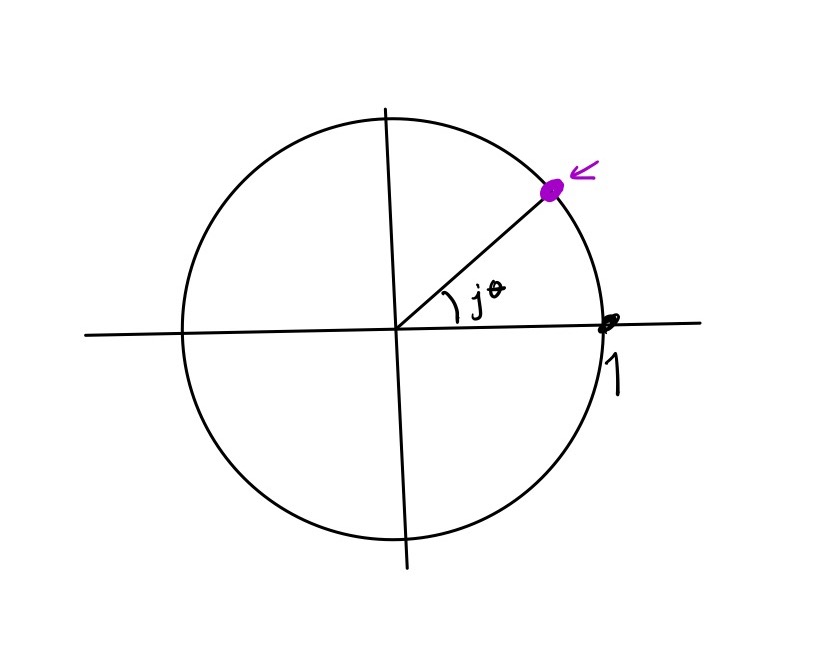
\includegraphics[width=90mm]{jtheta.jpg}
\caption{unit complex number at angle $j \theta$ \label{jtheta}}
\end{figure}

As described in Chapter~\ref{complex exponentials}, we may represent this complex number as
\[E[j] = e^{ij\theta} = \cos{j\theta} + i \sin{j \theta}.\]

Of course, since we are interested in periodic signals, we will require that $N\theta$ is a multiple of $2\pi$. We therefore have the following natural choices for $\theta$:
\[\theta = 0, 2 \pi/N, 4 \pi / N, \ldots, 2k\pi/N, \ldots, 2(N-1)\pi/N.\]
Note that it would serve no purpose to continue, as $2N\pi/N = 2\pi$ also corresponds to an angle of $0$.

We can represent these periodic signals as follows. Setting $E_k$ to be the signal with $\theta= 2k\pi/N$, we have:
\[E_k[j] = e^{ij\theta} = e^{ij2k\pi/N} = \left(e^{2\pi i / N}\right)^{jk}. \]
For convenience, we let $\omega = e^{2 \pi i / N}$, so that we may write our basic waveforms as:
\[E_k[j] = \omega^{jk} \]

The critical fact about these signals is that they also form a basis for the vector space of our periodic signals. That is, just as we may uniquely represent a signal $f$ as a linear combination of the signals $e_k$, we may also uniquely represent it is a linear combination of the signals $E_k$ as well. The change of basis matrix has a particularly nice form. It turns out to be equal to $1/N F_N$, where $F_N$ is the ``Fourier'' matrix. It's entries are given by $(F_N)_{k,j} = \omega^{-jk}$. That is, if we write $f = \sum f[k] e_k$, and do the matrix product:
\[
F_N
\left[
\begin{matrix}
	f[0] \\
	f[1] \\
	\vdots \\
	f[N-1]
\end{matrix}
\right]
=
\left[
\begin{matrix}
	\hat f[0] \\
	\hat f[1] \\
	\vdots \\
	\hat f[N-1]
\end{matrix}
\right]
\]

Then the coefficients $\hat f[k]$ of the resulting vector, which are called the \textbf{Fourier coefficients} of $f$, are related to expressing $f$ in terms of the basic waveforms as follows:
\begin{equation} \label{fourier basis expression}
f = \sum_k f[k] e_k = \sum \frac 1 N \hat f[k] E_k.
\end{equation}

\begin{prop} \label{fourier coeffs determine}
A signal is completely determined by its Fourier coefficients. That is, if two signals $f$ and $g$ satisfy $\hat f[k] = \hat g[k]$ for all $k$, then $f = g$.
\end{prop}
\begin{proof}
This follows from the fact that the Fourier coefficients directly determine the coefficients of a signal expressed as a vector in the basis of waveforms, by Equation~\ref{fourier basis expression}.
\end{proof}

The matrix $F_N$ (or rather the corresponding linear transformation) is called \textbf{Discrete Fourier Transform}, and the vector
\[\vec{\hat f} = F_N \vec f =
\left[
\begin{matrix}
	\hat f[0] \\
	\hat f[1] \\
	\vdots \\
	\hat f[N-1]
\end{matrix}
\right]
\]
is called the Fourier transform of $\vec f$. Note that since the Fourier coefficients are obtain by the application of a linear transformation, they satisfy
\begin{equation} \label{hat is linear}
\widehat{f + g}[k] = \hat f[k] + \hat g[k] \text{, and }\widehat{\lambda f}[k] = \lambda \hat f[k]
\end{equation}
for scalars $\lambda$.

\medskip
Let us work out the effect of this Fourier transform in some examples, starting with the standard basis signals $e_k$.
As the $k$'th column of the matrix $F_N$ represents the effect of the Fourier tranform on the $k$'th basis vector $\vec e_k$, we find that $F_N \vec e_k$ is represented by the column vector $\begin{bmatrix} \omega^{0} \\ \omega^{-k} \\ \omega^{-2k} \\ \vdots \\ \omega^{-(N-1)k} \end{bmatrix}$. Since by definition, these entries are the Fourier coefficients $\hat e_k[j]$, we find the useful fact:
\begin{equation} \label{fourier coeffs of std}
\boxed{\hat e_k[j] = \omega^{-jk}}
\end{equation}
Using Equation~\ref{fourier coeffs of std} and Equation~\ref{hat is linear}, we can give a formula for the Fourier coefficients of a general signal $f = \sum_k f[k] e_k$. For this, we obtain:
\begin{equation*}
\hat f[j] = \widehat{\left(\sum_k f[k] e_k\right)}[j] = \sum_k f[k] \hat e_k[j] = \sum_k f[k] \omega^{-jk}
\end{equation*}
and so
\begin{equation} \label{fourier coeffs formula}
\boxed{\hat f[j] = \sum_k f[k] \omega^{-jk}}
\end{equation}
Finally, let us compute the Fourier coefficients of the standard wave functions. For this, we will simply use the definition of the Fourier coefficients, and their relation to the change of basis. We have, by applying Equation~\ref{fourier basis expression} in the case $f = E_j$:
\begin{align*}
E_j &= \sum_k \frac{\hat E_j[k]}{N} E_k \\
&= \frac{\hat E_j[0]}{N} E_0 + \cdots +
\frac{\hat E_j[j-1]}{N} E_{j-1} + \frac{\hat E_j[j]}{N} E_{j} + \frac{\hat E_j[j+1]}{N} E_{j+1} + \cdots + \frac{\hat E_j[N-1]}{N} E_{N-1}
\end{align*}
But of course we can also write (trivially):
\begin{align*}
E_j &= 0 \cdot E_0 + \cdots +
0 \cdot E_{j-1} + 1 \cdot E_{j} + 0 \cdot E_{j+1} + \cdots + 0 \cdot E_{N-1}
\end{align*}

But since the signals $E_k$ form a basis, the expression for $E_j$ as a combination of the $E_k$'s is unique. Equating these gives:
\begin{equation} \label{fourier coeffs of waveforms}
\boxed{\hat E_j[k] = 0 \text{, if $k \neq j$, and } \hat E_j[j] = N}
\end{equation}

\section{Filters, circular convolution and circulant matrices}

In this section, we will take a look at the concept of filters from a few different computational vantage points. Filters represent a certain class of linear transformations, which take a signal and produce a new one with a modified frequency spectrum, amplifying certain frequencies, dampening others, and shifting the phase of some. Intuitively, these behave somewhat like an equalizer -- boosting the mid frequencies, while dampening the high ones, etc.

One subtelty of these ideas, is how these particular linear transformations are represeted in terms of different choices of bases. From the above description, it probably comes as no surprise that the description of a filter is represented particulalry easily in terms of the wave basis. Interestingly, there is another description, still fairly simple, in terms of the standard basis as well -- this involves the notion of convolution of functions. Finally, we will also explore another method of representing a filter, via a special class of matrices, called circulant matrices.

\subsection{Filters and Fourier coefficients}


As has been described, we think of a filter as a process which takes one function and modifies the waveforms which compose it by amplifying, damping or phase shifting. So, how does one specify a paricular rubric specifying how each waveforms is to be modified? Intuitively, one would want to associate a number to each basic waveform -- but in fact, this is nothing but a vector expressed in the wave basis, corresponding to another signal.

In summary, given a signal $f$, we can use $f$ as a template create a filter which modifies other signals. We use the following notations: for another signal $y$, we write
\[ T_f y  \text{ or } f * y \]
to represent the action of a filter, built from the waveforms arising in $f$, applied to $y$. These filters are defined in the following way:

\begin{defn} \label{filter def}
Given signals $f$ and $y$, we define $T_f y = f * y$ to be the unique the signal with Fourier coefficients:
\[ \widehat{f * y} [k] = \hat f[k] \hat y[k]. \]
\end{defn}
Note that this is a sufficient definition by Proposition~\ref{fourier coeffs determine}.

Let's think of what this means for a signals which have been written in the wave basis. Suppose that $f = \sum_k a_k E_k, y = \sum_k b_k E_k$. We will write $f * y = \sum_k c_k E_k$ and solve for the coefficients $c_k$ in terms of our expressions for $f$ and $y$. By Equation~\ref{fourier basis expression}, we may identify $\hat f[k] = N a_k, \hat y[k] = N b_k, \widehat{f * y}[k] = N c_k$. This tells us
\[ Nc_k = \widehat{f * y}[k] = \hat f[k] \hat y[k] = N^2 a_k b_k \]
which tells us
\begin{equation}
c_k = N a_k b_k
\end{equation}

To get a feeling for that, let's consider an example:

\begin{ex}
Let $N = 4$, $f = i E_0 - 2 E_1 + 3 E_2 + (2 - i) E_3$ and $y = 2 E_0 + E_1 - 5 E_2 - E_3$. We then have
\begin{align*}
f * y &= (4)(i)(2) E_0 + (4)(-2)(1) E_1 + (4)(3)(-5) E_2 + (4)(2 - i)(-1) E_3 \\
&= 8i E_0 - 8 E_1 - 60 E_2 + (-8 + 4i) E_3
\end{align*}
\end{ex}

\subsection{Filters and convolution}

Let us take a look at the effect of filtering in the standard basis. To aid us in our calculations, it will be useful to record a few facts about the filtering process.

\begin{prop}
Suppose we have signals $f, f_1, f_2, y, y_1, y_2$, and a scalar $\lambda$. Then:
\begin{gather*}
(f_1 + f_2) * y = f_1 * y + f_2 * y, \ f * (y_1 + y_2) = f * y_1 + f * y_2, \\ f * (\lambda y) = (\lambda f) * y = \lambda (f * y)
\end{gather*}
\end{prop}
These identities may be checked by comparing Fourier coefficients (by Proposition~\ref{fourier coeffs determine}). For example, for the first identity, we see by Definition~\ref{filter def} by Equation~\ref{hat is linear}, we have:
\begin{multline*}
\widehat{\left((f_1 + f_2)*y\right)}[k] = \widehat{(f_1 + f_2)}[k] \hat y[k] = (\hat{f_1}[k] + \hat{f_2}[k]) \hat y[k] = \hat f_1[k] \hat y[k] + \hat f_2 \hat y[k] \\
= \widehat{f_1 * y}[k] + \widehat{f_2 + y}[k]
\end{multline*}
and so, since this verifies that the signals $(f_1 + f_2)*y$ and $f_1 *y + f_2 * y$ have the same Fourier coefficients, they must be equal. The other identities may be checked similarly.

Let us now explore the effects of filtering in terms of the standard basis:
\begin{prop}
We have $e_k * e*j = e_{k+j}$, where $k + j$ is taken to be addition in $\mathbb Z/N\mathbb Z$. That is, we identify $0$ with $N$ with $2N$, we identify $1$ with $N+1$, etc.
\end{prop}
\begin{proof}
As before, we can verify this by comparing Fourier coefficents. By Definition~\ref{filter def}, the $\ell$'th Fourier coefficient of $e_k * e_j$ is computed as:
\[\widehat{e_k * e_j}[\ell] = \hat e_k[\ell] \hat e_j[\ell]\]
and by Equation~\ref{fourier coeffs of std}, this can be written as:
\[\hat e_k[\ell] \hat e_j[\ell] = \omega^{-k\ell} \omega^{-j\ell} = \omega^{-(j + k)\ell} = \hat e_{j+k}[\ell].\]
Therefore, the Fourier coefficients of $e_k * e_j$ and $e_{j+k}$ agree, and are therefore equal.
\end{proof}

From this, we obtain a very natural formula for the action of filtering. Given signals $f = \sum_k a_k e_k$ and $y = \sum_j b_j e_j$, (note that this means $f[k] = a_k$ and $y[j] = b_j$) we have
\[f * y = \left(\sum_k a_k e_k\right)*\left(\sum_j b_j e_j\right) = \sum_{j,k} a_k e_k * b_j e_j = \sum_{j,k} a_k b_j e_{k + j}.\]
We can obtain a formula written in a slightly different way by introducing a new variable $\ell$, and grouping terms of the form $e_\ell$ as follows:
\begin{equation} \label{convolution scratchwork}
f*y = \sum_{j,k}a_k b_j e_{k + j} = \sum_{\ell \in \mathbb Z/N\mathbb Z} \left(\sum_{\overset{j, k \in \mathbb Z/N\mathbb Z}{j + k = \ell}} a_k b_j\right)e_{\ell} = \sum_{\ell \in \mathbb Z/N\mathbb Z} \left(\sum_{k \in \mathbb Z/N\mathbb Z} a_kb_{N-k}\right)e_\ell
\end{equation}

This particular formula is also known as the \textbf{circular convolution}.

\begin{defn}
Let $f, y$ be signals. We define the circular convolution of $f \star y$ to be the signal with
\[(f \star y)[\ell] = \sum_{k\in \mathbb Z/N\mathbb Z} f[k]y[N-k].\]
\end{defn}

\begin{thm}
For signals $f, y$ we have $f * y = f \star y$.
\end{thm}
\begin{proof}
This follows from Equation~\ref{convolution scratchwork}.
\end{proof}

\iffalse
\section{The fast Fourier transform}
\fi

\appendix

\chapter{Complex exponentials}

\section{Complex arithmetic and polar form}

Although in typical applications, we deal with real numbers (to some fixed precision), allowing ourselves to work also with complex number can add a great variety of additional tools to bring to bear. In particular, we will eventually see that periodic functions, such as the sine and cosine, can be efficiently and compactly described via complex exponential functions, and doing this makes it a great deal more efficient decompose periodic signals into basic waveforms (i.e. via the Fourier transform).

Recall that a complex number $z = x + iy$, can be thought of graphically as a point in the complex plane, where we think of $x$ and $y$ as the coordinates of a point $(x, y)$. In this representation, it is clear that addition of complex numbers corresponds to addition of vectors -- that is
\[ (x_1 + i y_1) + (x_2 + i y_2) = (x_1 + x_2) + i (y_1 + y_2)\]
agrees with the vector sum
\[ (x_1, y_1) + (x_2, y_2) = (x_1 + x_2, y_1 + y_2) \]
But what about complex multiplication? For multiplication we see a nice visual interpretation by considering a polar representation of the complex number: if the point $(x_j, y_j)$, $j = 1, 2$ in the plane correpsonds to a vector of length $r_j$ and making an angle of $\theta_j$ with the positive $x$-axis, then we may write
\[z_j = x_j + i y_j = r_j \cos \theta_j + i r_j \sin \theta_j \]
and we find (using the sum formula for sine and cosine):

\begin{align} \label{angles add}
(x_1 + i y_1)(x_2 + i y_2) &= (r_1 \cos \theta_1 + i r_1 \sin \theta_1)(r_2 \cos \theta_2 + i r_2 \sin \theta_2) \\ &= r_1 r_2 \Big( (\cos \theta_1 \cos \theta_2 - \sin \theta_1 \sin \theta_2) (\cos \theta_1 \sin \theta_2 + \cos \theta_2 \sin \theta_1 )\Big) \\ &= r_1 r_2 \cos (\theta_1 + \theta_2) + i r_1 r_2 \sin (\theta_1 + \theta_2).
\end{align}

Said another way, we can visualize the multiplication of complex numbers in the following way: \textbf{lengths multiply and angles add}.

\section{Complex Exponentials} \label{complex exponentials}

We can view complex multiplication in a more intuitive light with the aid of Euler's formula, which gives a relationship between the complex exponential function and the polar representation of a complex number. Euler's formula states that for a real number\footnote{in fact the formula holds for complex numbers as well, and can be taken as a definition of cosine and sine for complex arguments} $\theta$, we have
\[e^{i \theta} = \cos \theta + i \sin \theta. \]
This formula can be verified by, for example, replacing each side by the corresponding power series expansions.

The complex exponential function -- that is, the function $e^z$ where $z$ can be any complex number, shares the usual familar properties with its real counterpart: $e^{z + w} = e^z e^w$, immediately giving again the multiplication rule from equation~\ref{angles add} above.

\iffalse
Let's visualize how the graph of the function $e^{i \theta}$ as a function of the real variable $\theta$.
\fi

\iffalse
Given a complex number, expressed as \[z = r \cos \theta + i r \sin \theta,\] we see that we can raise $z$ to positive integer powers by the formula
\[z^n = r^n \cos n\theta + i r^n \sin n\theta.\]
In particular, it makes sense to extend this definition and simply define the exponential $z^s$ for any real number $s$, by the formula
\[z^s = r^s \cos s\theta + i r^s \sin s\theta\]
\fi

\bibliographystyle{alpha}
\bibliography{citations}
\printindex

\end{document}
